% Manual LaTeX report, styled after HW/00/docs/answer/latex/answer_indented.tex.
\documentclass[12pt,a4paper,fontset=none]{ctexart}

\usepackage[left=2.7cm,right=2.7cm,top=2.5cm,bottom=2.5cm]{geometry}
\usepackage{amsmath, amssymb}
\usepackage{booktabs}
\usepackage[font=small,labelfont=bf,labelsep=quad]{caption}
\usepackage{graphicx}
\usepackage{float}
\usepackage{hyperref}
\usepackage{xcolor}
\usepackage{fancyvrb}
\usepackage{setspace}
\usepackage{tabularx}

\setmainfont{Noto Serif CJK SC}
\setCJKmainfont{Noto Serif CJK SC}
\setmonofont[Scale=0.9]{DejaVu Sans Mono}
\setCJKmonofont[Scale=0.9]{Noto Sans CJK SC}
\graphicspath{{../assets/}{../../../result/}{../../../results/}{../../../outputs/}}
\setstretch{1.36}
\AtBeginDocument{\zihao{-4}\selectfont}
\setlength{\parindent}{2em}
\setlength{\parskip}{0pt}
\setlength{\abovedisplayskip}{0.65\baselineskip}
\setlength{\belowdisplayskip}{0.65\baselineskip}
\captionsetup{skip=0.35\baselineskip}
\sloppy
\clubpenalty=10000
\widowpenalty=10000

\hypersetup{hidelinks}

\setcounter{secnumdepth}{3}
\setcounter{tocdepth}{2}
\renewcommand{\thesubsection}{\arabic{subsection}}
\renewcommand{\thesubsubsection}{\thesubsection.\arabic{subsubsection}}
\ctexset{
  subsection = {
    format = {\zihao{-3}\bfseries},
    aftername = {\quad},
    beforeskip = {1.0\baselineskip},
    afterskip = {0.45\baselineskip}
  },
  subsubsection = {
    format = {\zihao{4}\bfseries},
    aftername = {\quad},
    beforeskip = {0.75\baselineskip},
    afterskip = {0.25\baselineskip}
  }
}

\newcommand{\reportgroup}[1]{%
  \phantomsection\addcontentsline{toc}{section}{#1}%
  \begin{center}
    {\zihao{4}\bfseries #1\par}%
  \end{center}
  \vspace{0.65\baselineskip}%
}
\newcommand{\problem}[1]{\subsection{#1}}
\newcommand{\blocktitle}[1]{\subsubsection{#1}}
\newcommand{\codeinline}[1]{{\normalfont #1}}
\newcommand{\fileinline}[1]{{\urlstyle{same}\nolinkurl{#1}}}
\newcommand{\metadataline}[1]{\makebox[\linewidth][l]{#1}}
\newcommand{\scriptpath}[1]{\fileinline{#1}}
\newcommand{\githubscriptsbase}{https://github.com/Void0312Aurora/computational-physics-homework-2026/blob/main/05/scripts}
\newcommand{\scriptlink}[1]{\noindent\metadataline{\textbf{相关脚本：}\href{../../../scripts/#1}{本地 \scriptpath{scripts/#1}} / \href{\githubscriptsbase/#1}{GitHub \scriptpath{scripts/#1}}}\par\medskip}
\DefineVerbatimEnvironment{CodeBlock}{Verbatim}{
  fontsize=\footnotesize,
  frame=single,
  framesep=0.5em,
  xleftmargin=1.2em,
  xrightmargin=1.2em
}

\title{\vspace{-1.0em}{\bfseries\zihao{3} HW06 课堂作业报告}\\[0.35em]{\zihao{-4} 插值方法与高精度圆周率计算实验报告：段首缩进版}}
\author{\zihao{-4} 姜玥晟}
\date{\zihao{-4} 2026-04-21}

\begin{document}
\pagestyle{plain}
\maketitle

\begin{figure}[H]
  \centering
  
\includegraphics[width=0.18\linewidth]{profile.jpg}
\end{figure}

\begin{table}[H]
  \centering
  \begin{tabular}{ll}
    \toprule
    项目 & 内容 \\
    \midrule
    项目目录 & \codeinline{HW/05} \\
    提交编号 & \codeinline{HW06} \\
    学生姓名 & 姜玥晟 \\
    报告主题 & 分段插值、Runge 现象、Neville 递推与高精度圆周率计算 \\
    实验环境 & \codeinline{Python} 插值程序、\codeinline{GMP}/GPU 高精度后端与 benchmark 数据 \\
    \bottomrule
  \end{tabular}
\end{table}

\newpage

\renewcommand{\contentsname}{目录}
\begingroup
\hypersetup{linkcolor=black}
\tableofcontents
\thispagestyle{plain}
\endgroup

\newpage

\reportgroup{I. 稳压二极管数据的分段插值}

给定 7 个稳压二极管电压-电流数据点：
\begin{table}[H]
  \centering
  \begin{tabular}{lrrrrrrr}
    \toprule
    Voltage & -1.00 & 0.00 & 1.27 & 2.55 & 3.82 & 4.92 & 5.02 \\
    Current & -14.58 & 0.00 & 0.00 & 0.00 & 0.00 & 0.88 & 11.17 \\
    \bottomrule
  \end{tabular}
\end{table}
题目指出，用一个整体 6 次多项式将全部 7 点连接起来会在点间产生明显摆动，因此应改用由低阶多项式组成的分段插值曲线。

\problem{Problem 1(1)：整体高阶插值的局限}
\scriptlink{problem1.py}

\blocktitle{待求问题}
说明整体 6 次多项式为何不适合这组数据。

\blocktitle{解决方式}
本小问只构造经过全部 7 个数据点的整体 6 次插值多项式 \(P_6(x)\)。由于 7 个互异节点唯一确定一个次数不超过 6 的插值多项式，这里使用 Neville 递推在致密网格和各区间中点上求值：
\begin{CodeBlock}
Input : sample points (x_i, y_i)
Output: global degree-6 interpolation values

build dense grid X
for each x in X do
    y_global <- Neville(all points, x)
end for

compute min, max and range of y_global
evaluate y_global at each interval midpoint
plot P_6(x) with the original data points
\end{CodeBlock}
Neville 递推不需要显式解 Vandermonde 方程，但得到的是同一个全局 \(P_6(x)\)。本小问不引入分段线性或 PCHIP，因为它要检验的正是整体 6 次多项式自身的点间行为。

\blocktitle{问题答案}
整体 6 次插值结果见图~\ref{fig:p1_global}。
\begin{figure}[H]
  \centering
  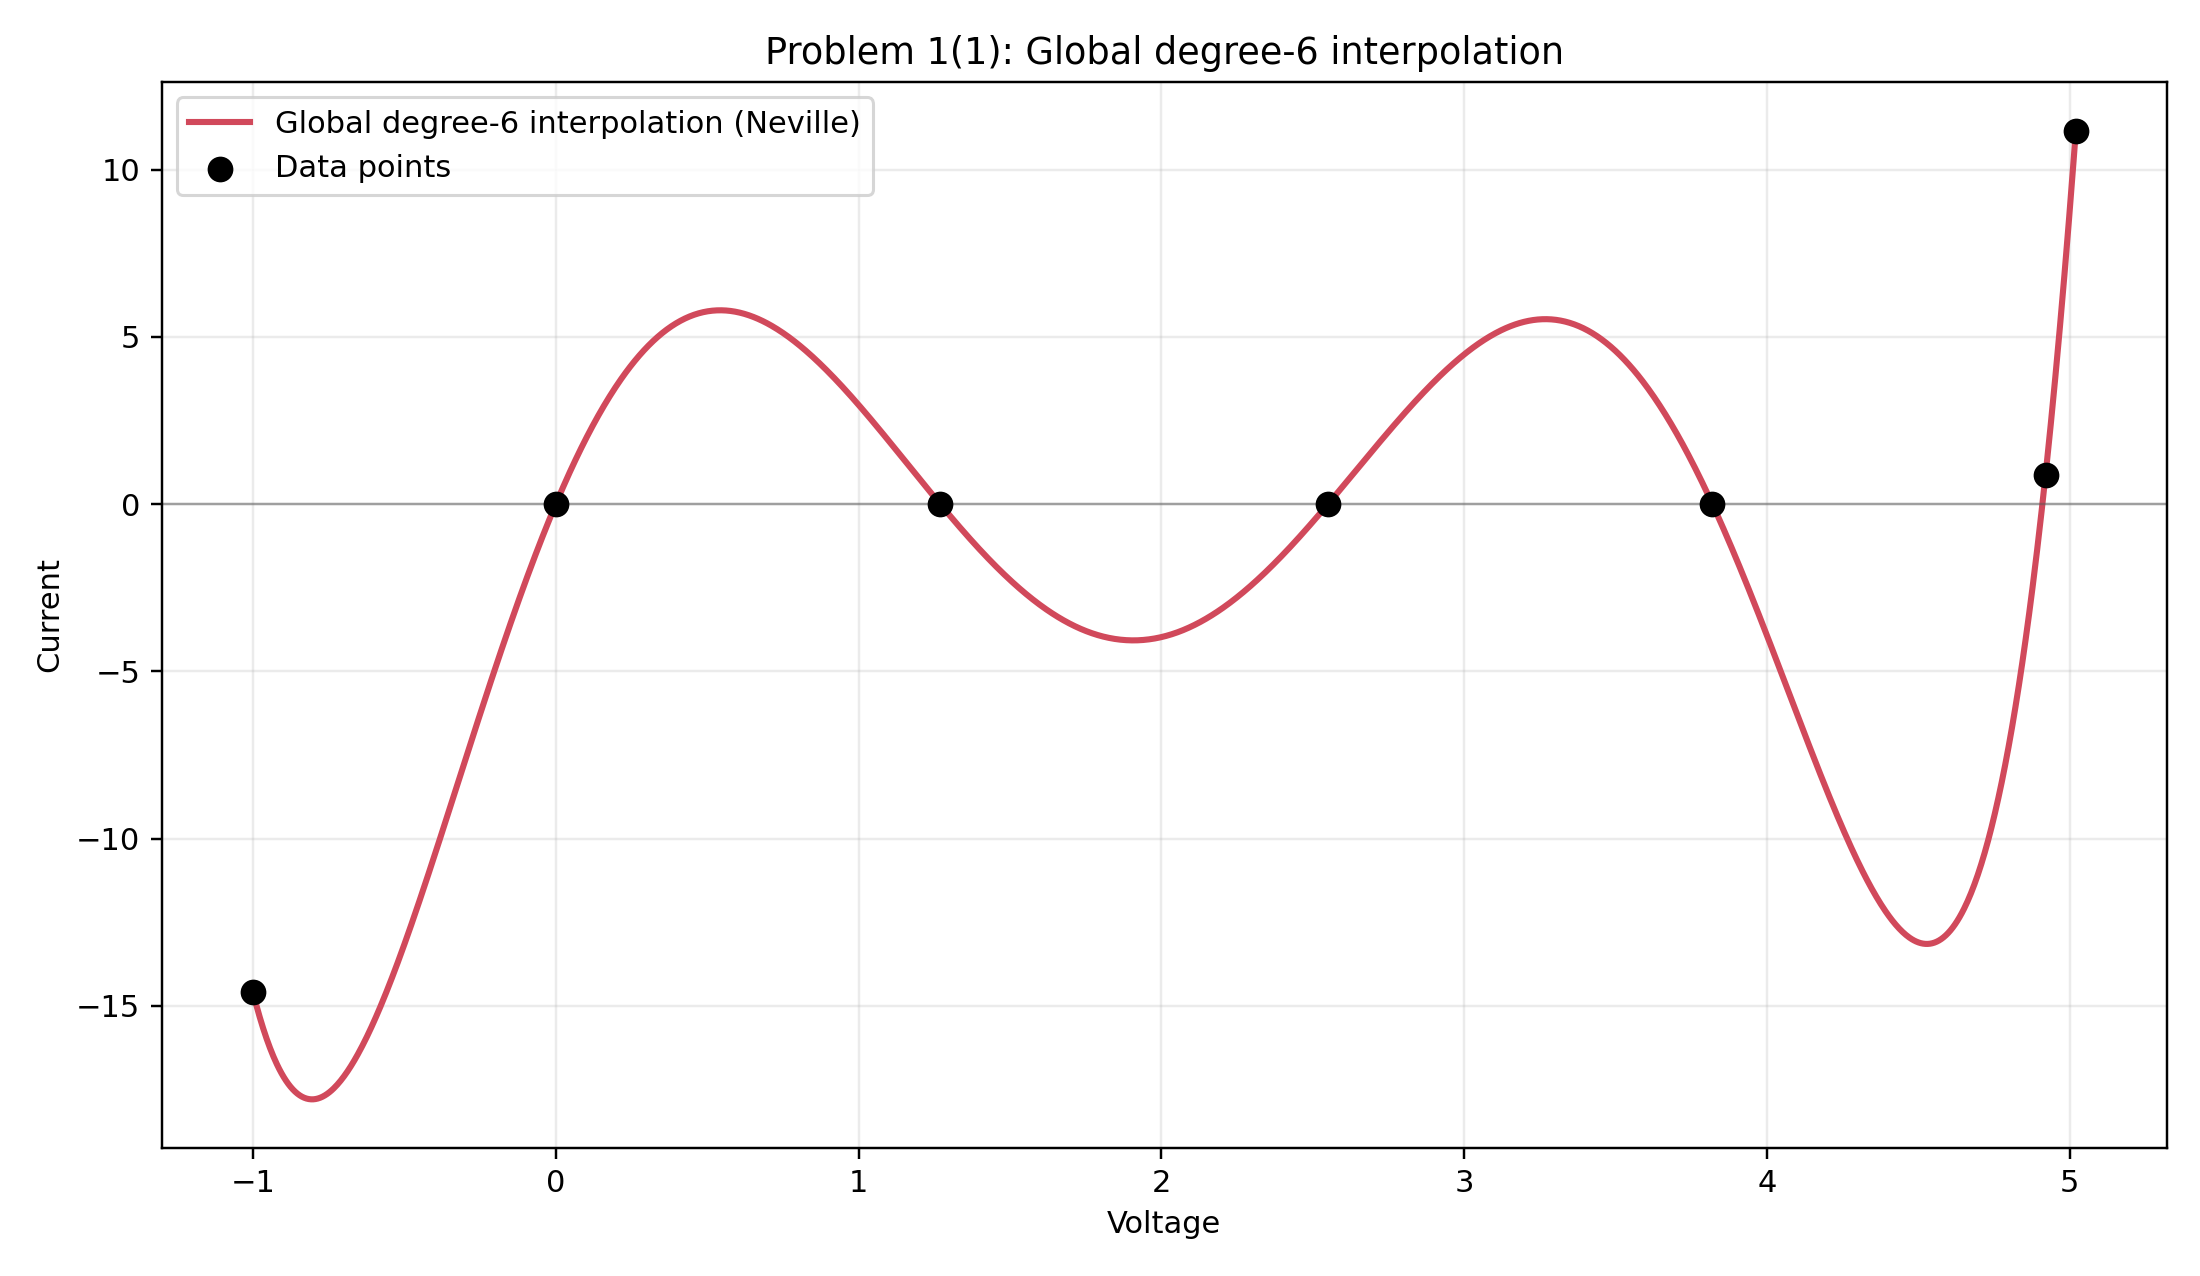
\includegraphics[width=0.94\linewidth]{problem1_global_degree6.png}
  \caption{稳压二极管数据的整体 6 次插值结果。}
  \label{fig:p1_global}
\end{figure}

\begin{table}[H]
  \centering
  \caption{整体 6 次插值与原始数据范围比较。}
  \begin{tabular}{lrrr}
    \toprule
    对象 & 最小电流 & 最大电流 & 振幅宽度 \\
    \midrule
    原始数据范围 & -14.580000 & 11.170000 & 25.750000 \\
    整体 6 次多项式 & -17.791266 & 11.170000 & 28.961266 \\
    \bottomrule
  \end{tabular}
\end{table}

\begin{table}[H]
  \centering
  \caption{整体 6 次插值在代表性中点的电流值。}
  \begin{tabular}{rr}
    \toprule
    中点电压 & 整体 6 次插值电流 \\
    \midrule
    -0.500 & -13.161141 \\
    0.635 & 5.656649 \\
    1.910 & -4.070359 \\
    3.185 & 5.421118 \\
    4.370 & -11.866745 \\
    4.970 & 5.566334 \\
    \bottomrule
  \end{tabular}
\end{table}
由此可见，整体 6 次多项式在平台段附近产生了明显的虚假振荡。原始数据电流范围是 \codeinline{25.75}，而 \(P_6(x)\) 的范围扩大到 \codeinline{28.961266}；在实际应接近零的平台区间，中点 \codeinline{0.635}、\codeinline{1.910}、\codeinline{3.185} 处分别给出 \codeinline{5.656649}、\codeinline{-4.070359}、\codeinline{5.421118}。因此，整体 6 次多项式虽然严格通过所有节点，但不适合表示这组二极管伏安曲线。

\blocktitle{理解}
本小问说明的是整体高阶插值的失败原因。稳压二极管数据同时包含平台段和陡升段，整体 \(P_6(x)\) 被迫用一组全局系数同时满足所有节点，因此远端节点会影响平台段形状，产生不符合物理直觉的点间过冲。问题不在于它是否通过数据点，而在于通过数据点之间的连续曲线是否可信。

\problem{Problem 1(2)：分段插值方案}
\scriptlink{problem1.py}

\blocktitle{待求问题}
构造由低阶多项式组成的分段插值曲线，并给出比较。

\blocktitle{解决方式}
本小问不再使用整体 \(P_6(x)\)，而是在每个相邻节点区间内单独构造低阶多项式。本文采用两条分段曲线：分段线性作为最低阶保守方案，保形三次 Hermite/PCHIP 作为更平滑的低阶方案。
\begin{CodeBlock}
Input : sample points (x_i, y_i)
Output: low-order piecewise interpolation curves

for each interval [x_i, x_{i+1}] do
    y_linear <- line segment through the two endpoints
    y_pchip <- cubic Hermite segment with shape-preserving slopes
end for

compute range and midpoint values of both piecewise curves
plot only the low-order piecewise curves with data points
\end{CodeBlock}
对 PCHIP，记
\[
  h_i=x_{i+1}-x_i,\qquad \delta_i=\frac{y_{i+1}-y_i}{h_i}.
\]
当相邻割线斜率 \(\delta_{i-1}\) 与 \(\delta_i\) 异号或其中一个为零时，令节点导数 \(m_i=0\)，避免在平台段人为制造过冲；当二者同号时，采用加权调和平均
\[
  m_i=\frac{w_1+w_2}{w_1/\delta_{i-1}+w_2/\delta_i},\qquad
  w_1=2h_i+h_{i-1},\quad w_2=h_i+2h_{i-1}.
\]
因此，低阶分段方案只受相邻或近邻节点控制，不会像整体 6 次多项式那样让远端节点共同影响平台段。

\blocktitle{问题答案}
低阶分段插值结果见图~\ref{fig:p1_piecewise}。两种分段方案都没有超过原始数据的电流范围，曲线最小值保持为 \codeinline{-14.58}，最大值保持为 \codeinline{11.17}。

\begin{figure}[H]
  \centering
  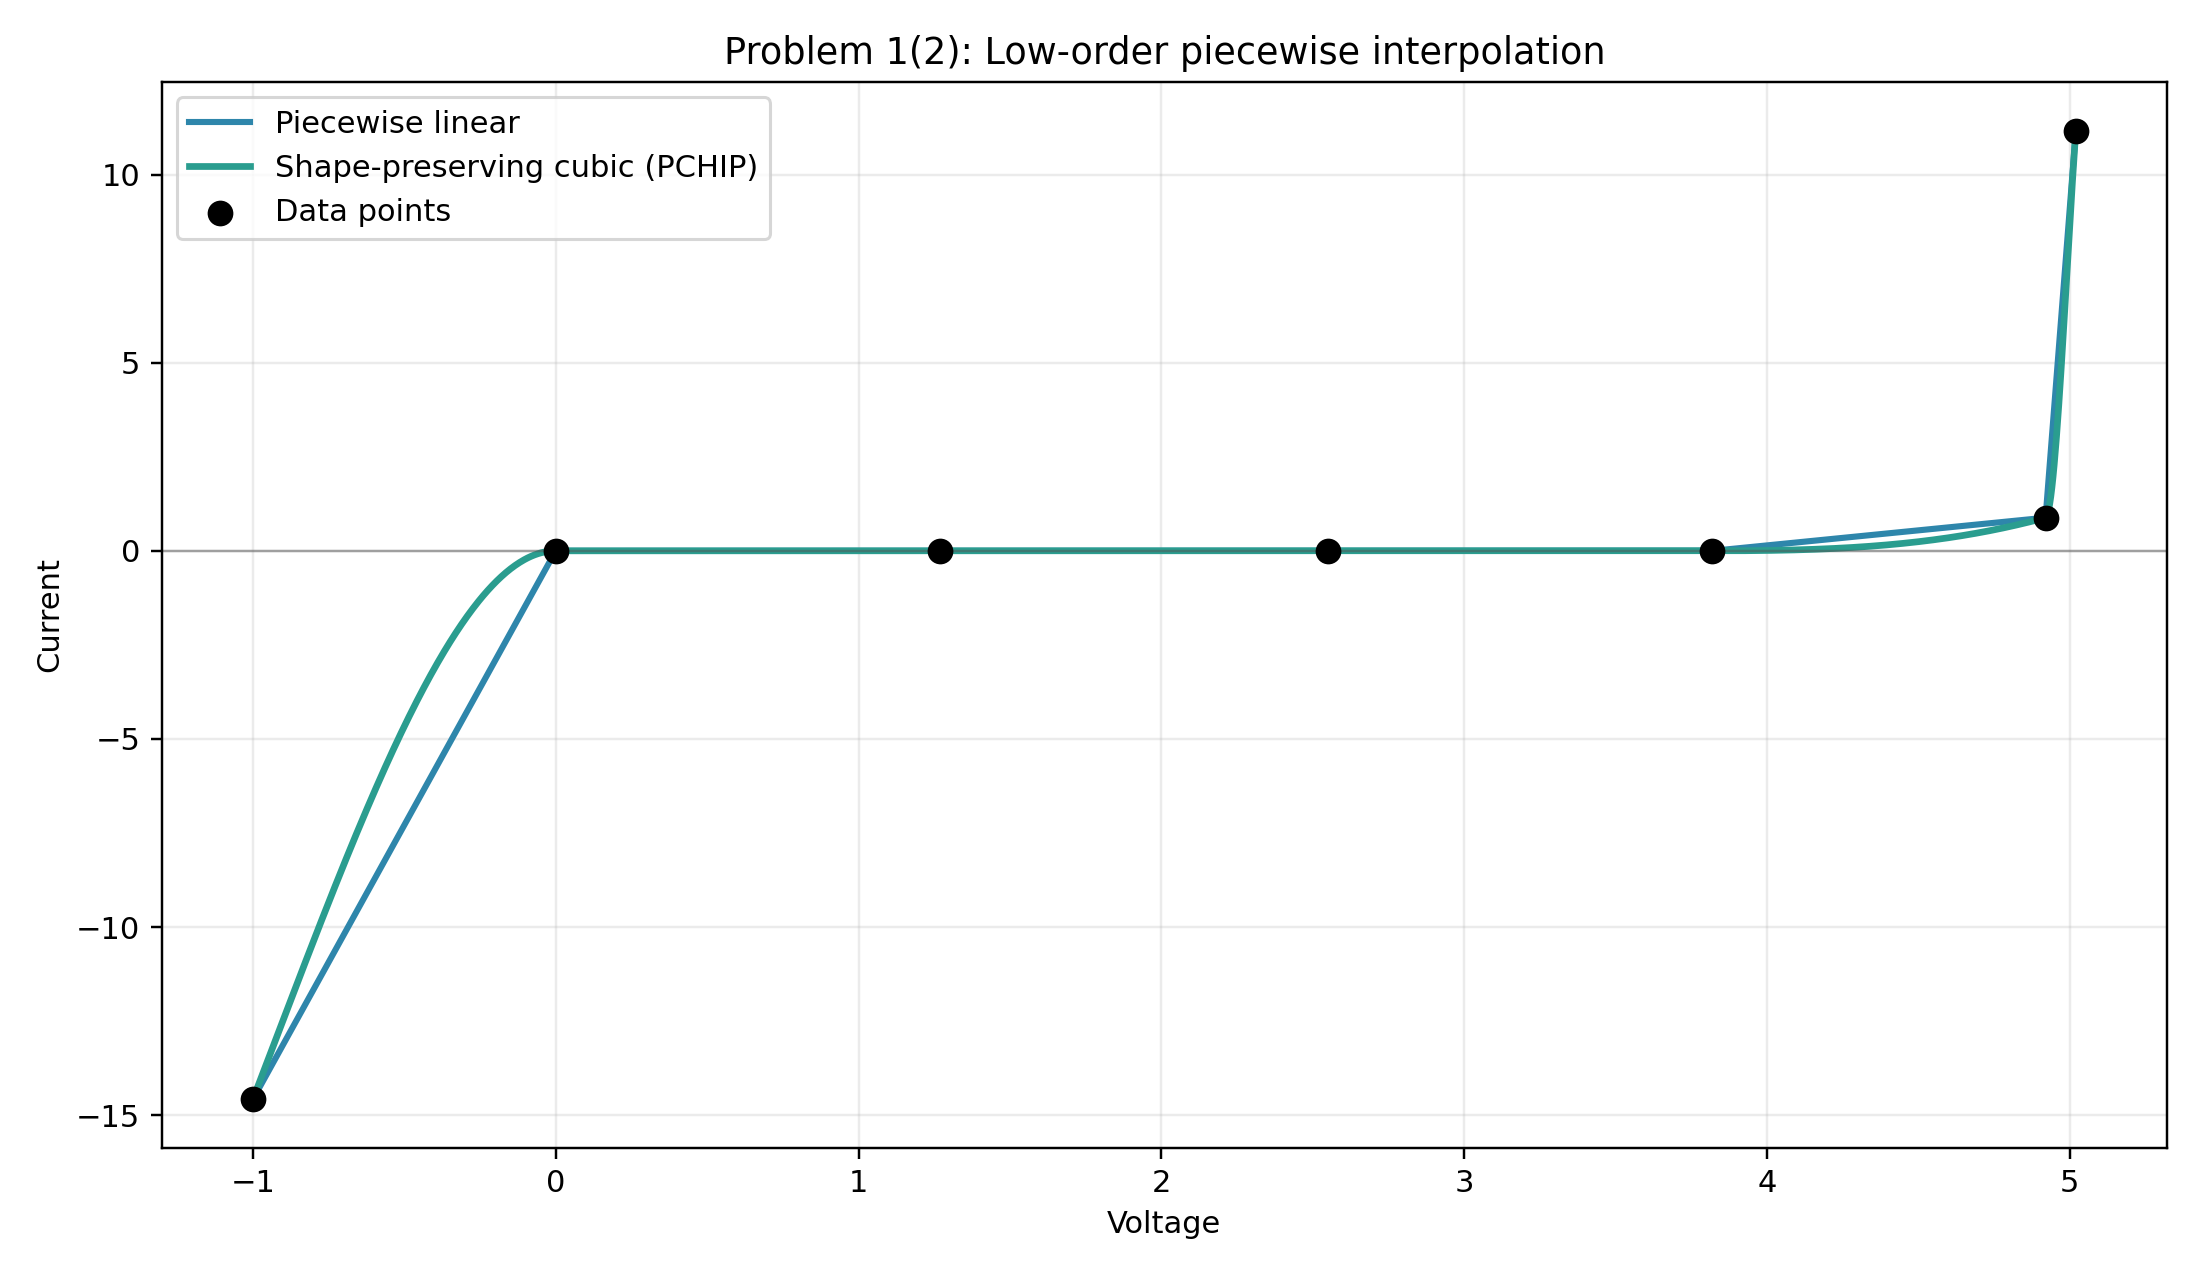
\includegraphics[width=0.94\linewidth]{problem1_piecewise_low_order.png}
  \caption{稳压二极管数据的低阶分段插值结果。}
  \label{fig:p1_piecewise}
\end{figure}

\begin{table}[H]
  \centering
  \caption{分段插值方案的电流范围。}
  \begin{tabular}{lrrr}
    \toprule
    分段方案 & 最小电流 & 最大电流 & 振幅宽度 \\
    \midrule
    分段线性 & -14.580000 & 11.170000 & 25.750000 \\
    保形三次 Hermite/PCHIP & -14.580000 & 11.170000 & 25.750000 \\
    \bottomrule
  \end{tabular}
\end{table}

\begin{table}[H]
  \centering
  \caption{分段插值在代表性中点的结果。}
  \begin{tabular}{rrr}
    \toprule
    中点电压 & 分段线性 & 保形三次 \\
    \midrule
    -0.500 & -7.290000 & -4.664637 \\
    0.635 & 0.000000 & 0.000000 \\
    1.910 & 0.000000 & 0.000000 \\
    3.185 & 0.000000 & 0.000000 \\
    4.370 & 0.440000 & 0.139518 \\
    4.970 & 6.025000 & 4.659712 \\
    \bottomrule
  \end{tabular}
\end{table}

由表中结果可见，分段线性在每个区间内直接连接相邻数据点，因此完全不会越过相邻节点范围；PCHIP 在平台段中点 \codeinline{0.635}、\codeinline{1.910}、\codeinline{3.185} 仍给出 \codeinline{0.000000}，同时在陡升段给出更平滑的过渡，例如 \codeinline{4.970} 处为 \codeinline{4.659712}。因此，分段线性适合作为保守基线，PCHIP 是本题更平滑且仍保持形状约束的分段插值结果。

\blocktitle{理解}
分段低阶插值将全局约束转化为局部约束，更适合这类具有明显分段物理特征的数据；若希望曲线比折线更光滑，同时又不牺牲平台段的形状约束，PCHIP 是本题中更合适的折中方案。

\reportgroup{II. Runge 函数上的等距节点插值}

对 Runge 函数
\[
  f(x)=\frac{1}{1+16x^2},
\]
在区间 \codeinline{[-1,1]} 上取等距节点。

\problem{Problem 2(1)：5 个节点的 5 次插值}
\scriptlink{problem2.py}

\blocktitle{待求问题}
先从 \codeinline{5} 个节点开始作图，并与精确函数进行比较。

\blocktitle{解决方式}
题面写作“\codeinline{5} 个等距点、\codeinline{5} 次多项式”，但从插值问题的良定性看，$m$ 个互异节点唯一确定的是次数不超过 $m-1$ 的插值多项式；若强行使用 $m$ 次多项式，还需要额外约束才能唯一确定。因此本文按节点数解释题意，本小问的 \codeinline{5} 个节点对应 4 次插值多项式。

本小问只计算 \codeinline{5} 个等距节点的插值曲线和误差指标：
\begin{CodeBlock}
Input : node count m = 5 and Runge function f(x)
Output: interpolation curve and error metrics

build 5 equispaced nodes on [-1, 1]
evaluate nodal data f(x_j)
for each query point x do
    y_neville <- Neville(nodes, values, x)
    y_bary <- barycentric_lagrange(nodes, values, x)
end for
compare interpolation with exact function
record max_abs_error and RMSE
\end{CodeBlock}
其中 Neville 递推负责生成报告中的插值曲线，重心 Lagrange 用于一致性核对。两种方法应给出同一个 4 次插值多项式；若二者差异只在舍入误差量级，说明实现没有把插值公式本身写错。

\blocktitle{问题答案}
5 个节点的插值结果见图~\ref{fig:p2_5}。
\begin{figure}[H]
  \centering
  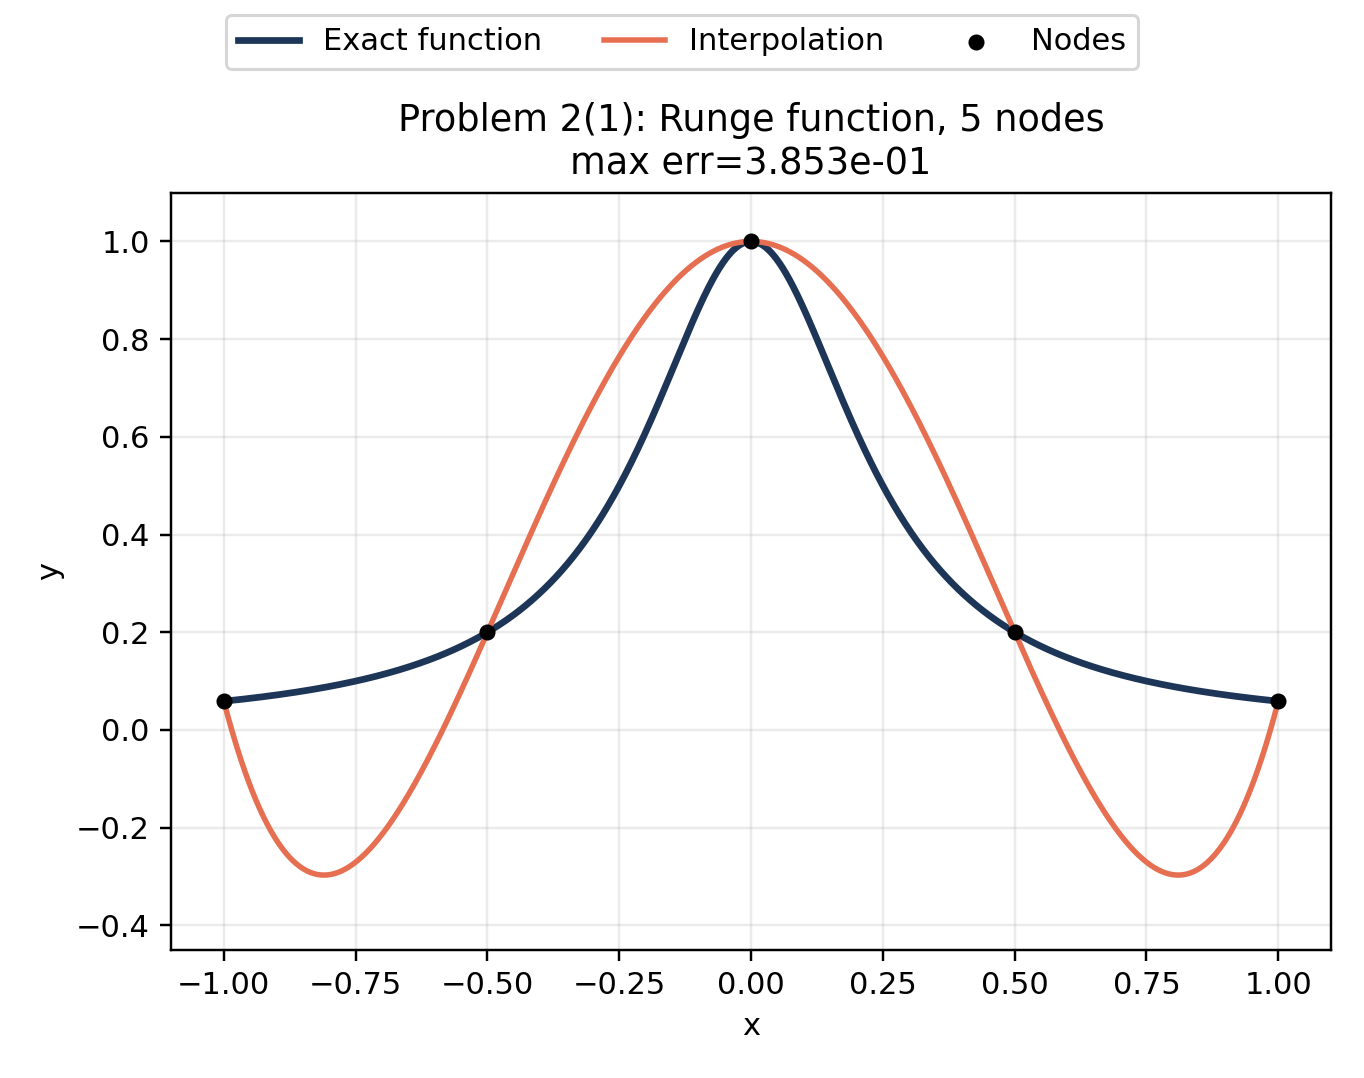
\includegraphics[width=0.94\linewidth]{problem2_runge_5_nodes.png}
  \caption{Runge 函数 5 个等距节点插值结果。}
  \label{fig:p2_5}
\end{figure}

\begin{table}[H]
  \centering
  \caption{Runge 函数 5 个节点插值误差。}
  \begin{tabular}{rrrr}
    \toprule
    节点数 & 插值次数 & 最大绝对误差 & RMSE \\
    \midrule
    5 & 4 & 3.853043e-01 & 2.316902e-01 \\
    \bottomrule
  \end{tabular}
\end{table}
由图和表可见，\codeinline{5} 个节点时已经能够观察到端点附近的偏离，但整体振荡尚未失控。该 4 次插值多项式的最大绝对误差为 \codeinline{3.853043e-01}，RMSE 为 \codeinline{2.316902e-01}；Neville 与重心 Lagrange 的最大逐点差异仅为 \codeinline{4.44e-16}，说明本小问的误差主要来自等距节点插值本身，而不是两种求值公式不一致。

\blocktitle{理解}
本小问作为基线实验，说明少量等距节点下 Runge 函数已经存在边界误差，但还没有出现后续高阶情形中的灾难性端点振荡。它为下一小问观察误差随节点数 \(b\) 增大而变化提供了基准。

\problem{Problem 2(2)：更多节点的重复实验}
\scriptlink{problem2.py}

\blocktitle{待求问题}
再对 \codeinline{7,9,17,19,21} 个节点重复，观察等距高阶插值的表现。

\blocktitle{解决方式}
本小问沿用上一小问的良定解释：$m$ 个等距节点生成次数不超过 $m-1$ 的插值多项式。继续增加节点数的目的不是改变插值公式，而是观察等距高阶插值在 Runge 函数上的误差传播。
\begin{CodeBlock}
Input : node counts M = [7, 9, 17, 19, 21]
Output: interpolation curves, error-vs-b curve and error table

for each m in M do
    build m equispaced nodes on [-1, 1]
    evaluate interpolation by Neville recursion
    evaluate interpolation by barycentric Lagrange
    compare interpolation with exact function
    record max_abs_error and RMSE
end for
\end{CodeBlock}
本实验中 Neville 与重心 Lagrange 最大逐点差异为 \codeinline{1.96e-11}，远小于 Runge 现象导致的函数逼近误差。

\blocktitle{问题答案}
更多节点的插值结果见图~\ref{fig:p2_more}。其中 \(b\) 表示等距节点数，最大误差与 RMSE 随 \(b\) 增大的变化见图~\ref{fig:p2_error_b}。
\begin{figure}[H]
  \centering
  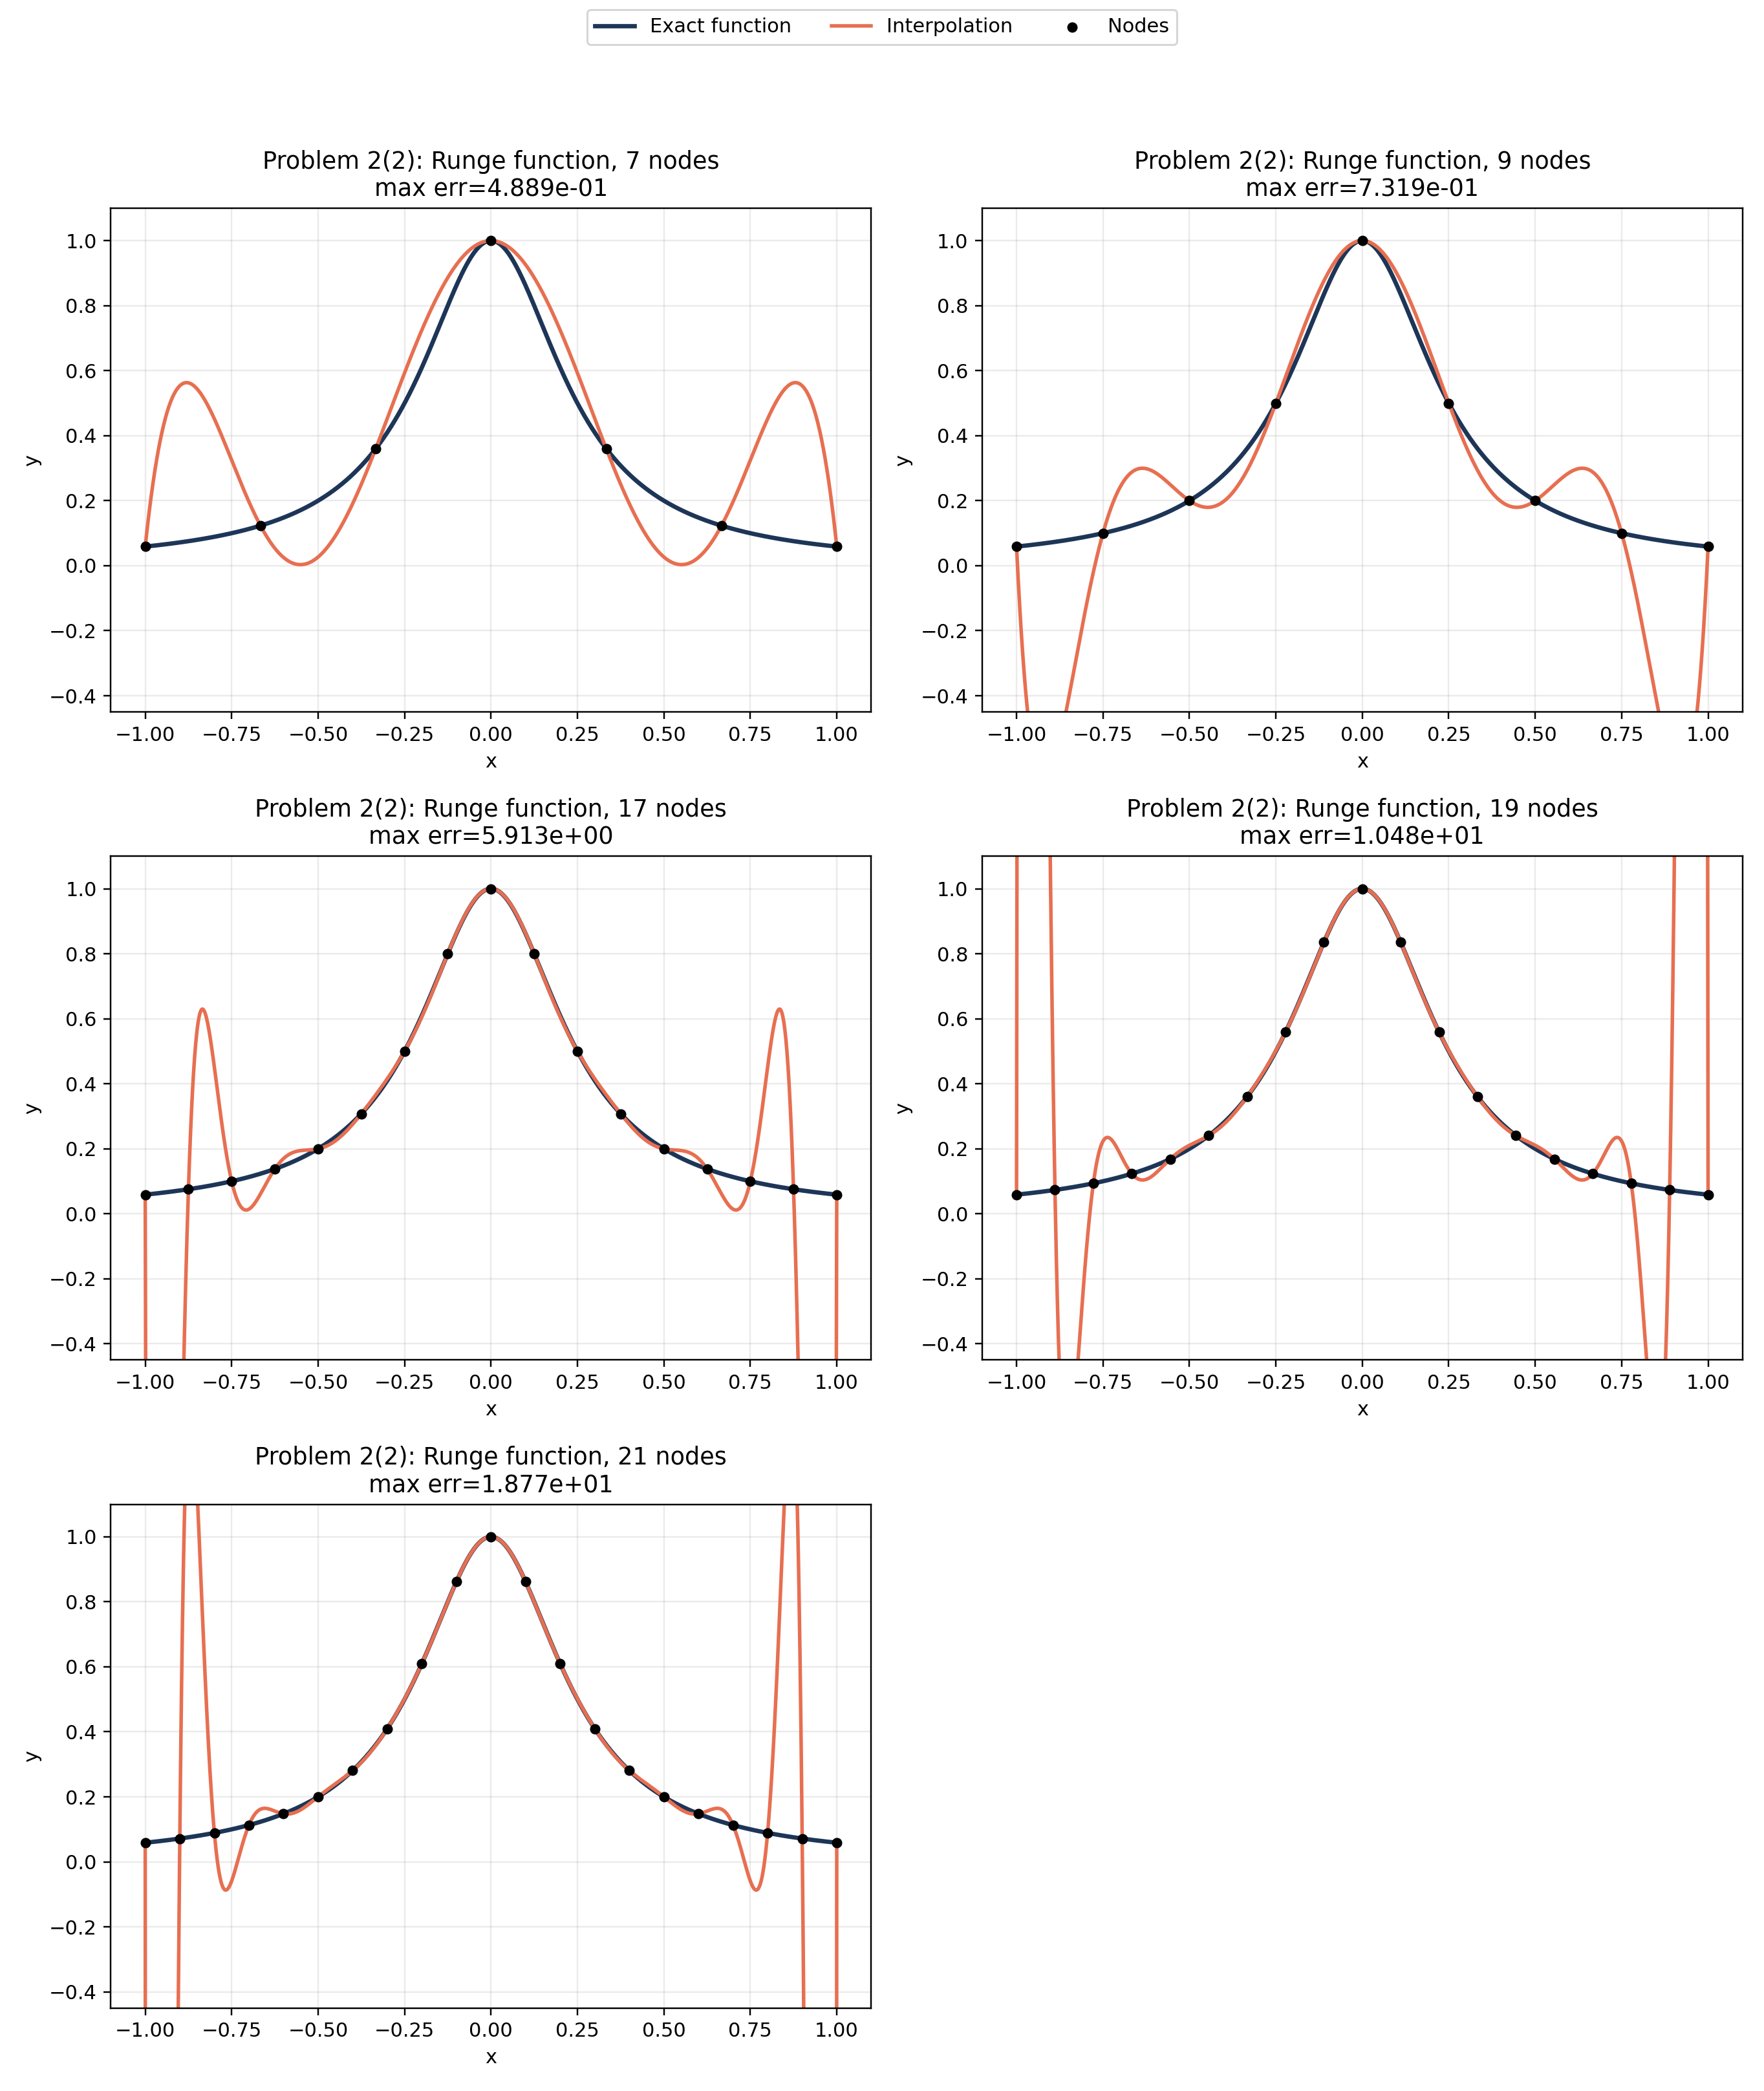
\includegraphics[width=0.99\linewidth]{problem2_runge_more_nodes.png}
  \caption{Runge 函数更多等距节点插值结果。}
  \label{fig:p2_more}
\end{figure}

\begin{figure}[H]
  \centering
  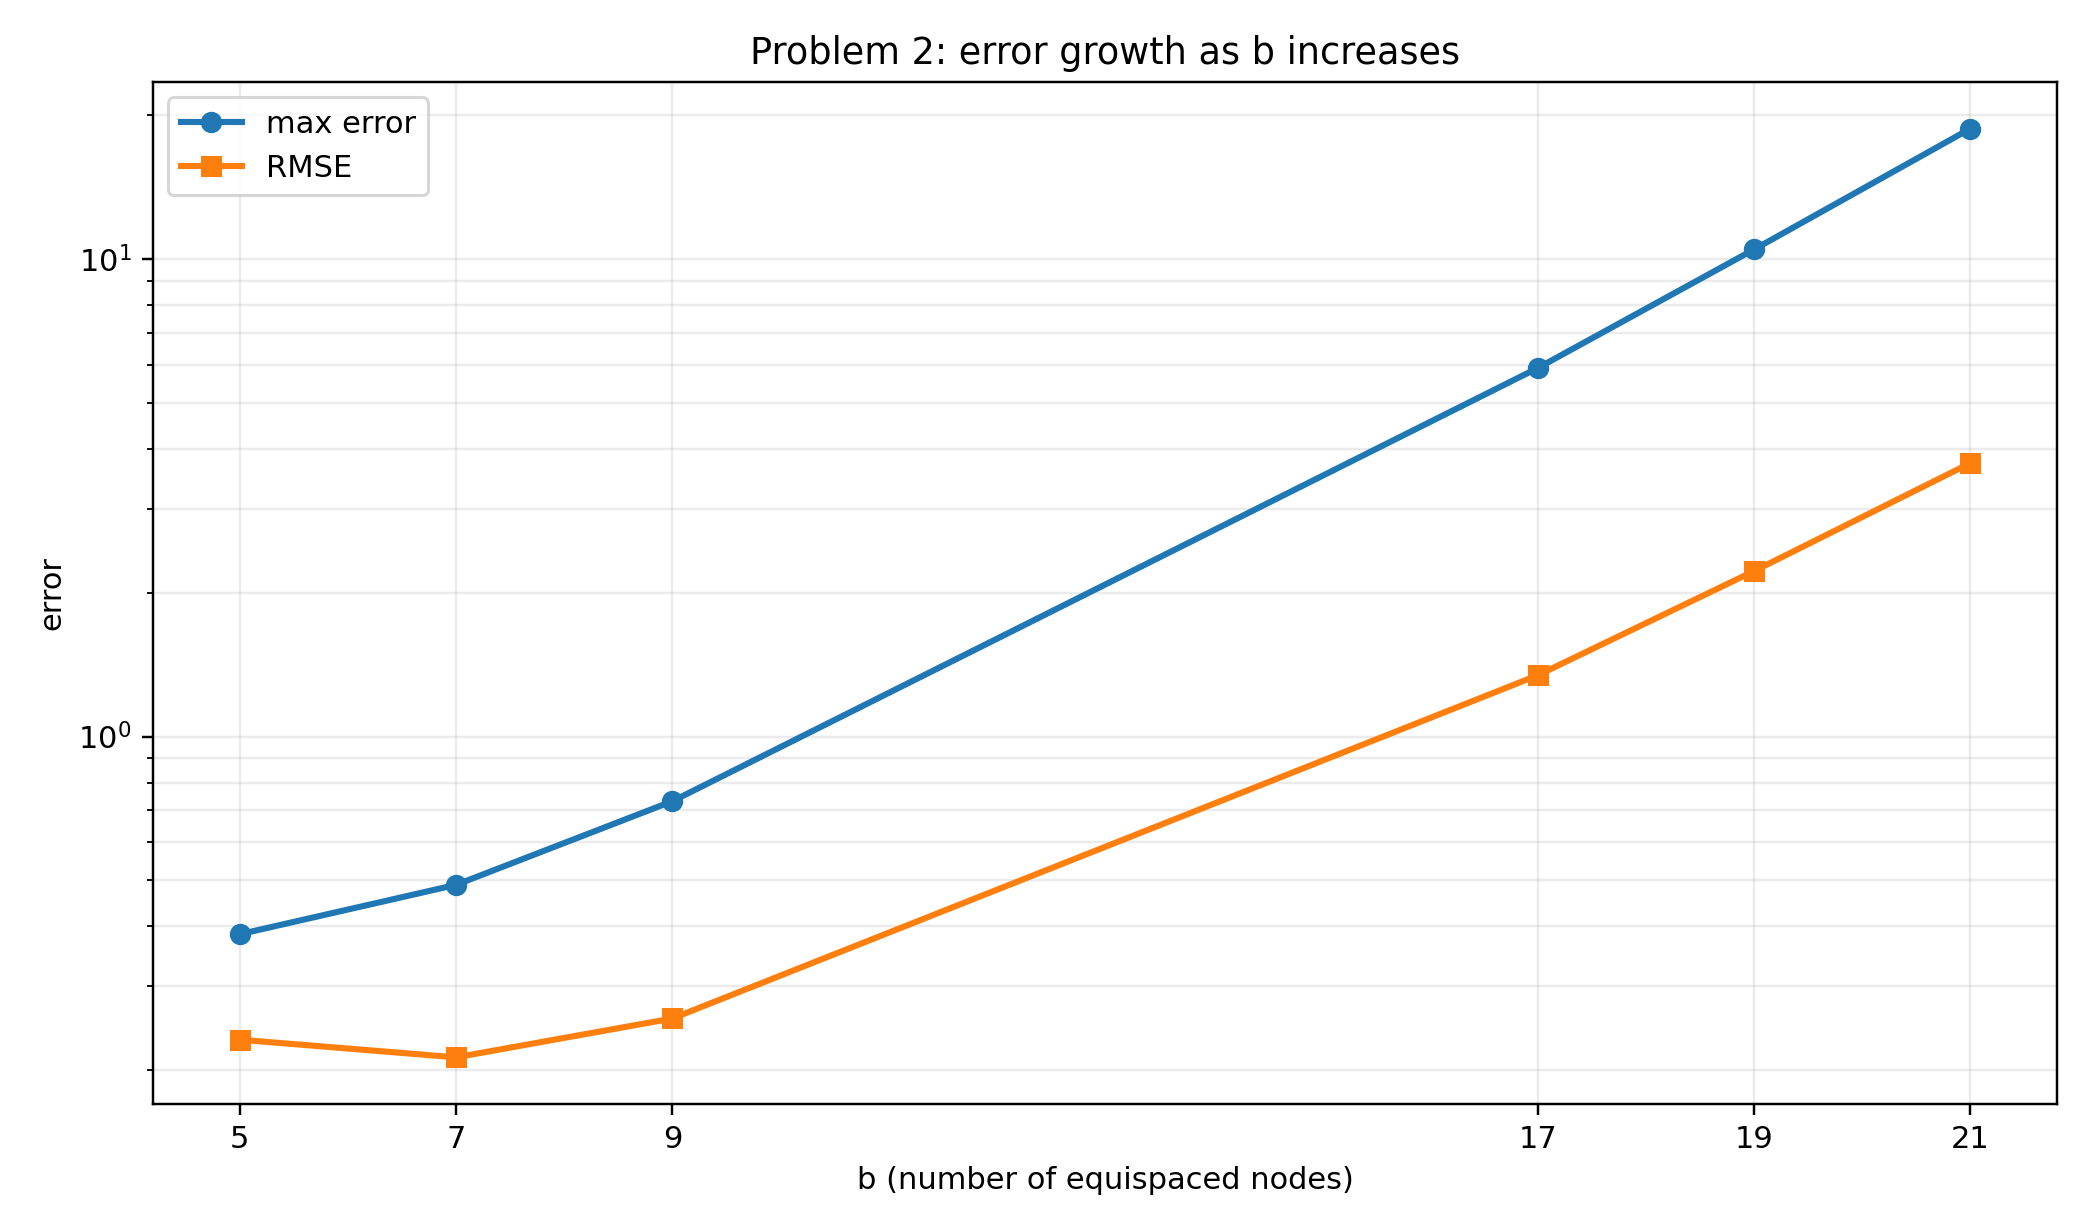
\includegraphics[width=0.90\linewidth]{problem2_runge_error_vs_b.png}
  \caption{Runge 函数插值误差随节点数 \(b\) 增大的变化。}
  \label{fig:p2_error_b}
\end{figure}

\begin{table}[H]
  \centering
  \caption{Runge 函数更多节点插值误差。}
  \begin{tabular}{rrrr}
    \toprule
    节点数 & 插值次数 & 最大绝对误差 & RMSE \\
    \midrule
    7 & 6 & 4.888773e-01 & 2.127766e-01 \\
    9 & 8 & 7.318894e-01 & 2.566409e-01 \\
    17 & 16 & 5.913241e+00 & 1.343585e+00 \\
    19 & 18 & 1.047845e+01 & 2.221318e+00 \\
    21 & 20 & 1.876836e+01 & 3.739459e+00 \\
    \bottomrule
  \end{tabular}
\end{table}
Neville 与重心 Lagrange 的逐点差异始终维持在机器精度附近，说明两种实现确实在求同一个插值多项式。继续增加节点数后，最大误差从 \codeinline{4.888773e-01} 增至 \codeinline{1.876836e+01}，RMSE 从 \codeinline{2.127766e-01} 增至 \codeinline{3.739459e+00}；图~\ref{fig:p2_error_b} 直接显示误差指标随 \(b\) 增大而上升。

\blocktitle{理解}
本题展示了经典的 Runge 现象。问题的根源不在于插值公式本身，而在于“等距节点 + 高阶整体多项式”这一组合对边界非常敏感。对 $b$ 个节点的插值多项式 $p_{b-1}$，误差可以写成
\[
  f(x)-p_{b-1}(x)=\frac{f^{(b)}(\xi_x)}{b!}\prod_{j=0}^{b-1}(x-x_j).
\]
这个公式说明误差由两部分共同决定：节点多项式 $\omega_b(x)=\prod_j(x-x_j)$ 的放大形态，以及目标函数高阶导数的增长速度。Runge 函数
\[
  f(x)=\frac{1}{1+16x^2}
\]
在复平面最近的奇点是 $x=\pm i/4$，距离实区间很近。按 Bernstein 椭圆估计，对应参数约为
\[
  \rho=\frac14+\sqrt{1+\frac1{16}}\approx 1.2808,
\]
因此最优多项式逼近的解析衰减尺度只有 $\rho^{-b}\approx e^{-0.247b}$。等距插值的稳定性因子却会随 $b$ 近似指数增长；当这个放大超过函数可逼近性的衰减时，整体误差就会随节点数增加而增大。

用表中 \codeinline{b=7,9,17,19,21} 的数据作半对数拟合，
\[
  E_\infty(b)\approx 7.36\times10^{-2}e^{0.261b},\qquad
  E_2(b)\approx 4.45\times10^{-2}e^{0.206b},
\]
其中 $E_\infty$ 表示最大误差，$E_2$ 表示 RMSE。两个拟合的 $R^2$ 分别为 \codeinline{0.9988} 和 \codeinline{0.9932}。这意味着在本实验范围内，每增加 1 个等距节点，最大误差平均乘以 \codeinline{1.30}，RMSE 平均乘以 \codeinline{1.23}。所以 \codeinline{21} 个节点的最大误差比 \codeinline{5} 个节点大约 \codeinline{48.7} 倍并不是偶然数值波动，而是“近奇点 + 等距高阶插值放大”共同作用的结果；若改用 Chebyshev 节点，这一放大会显著缓解。

\reportgroup{III. 振荡函数的等距节点插值}

对函数
\[
  f(x)=x\sin(2\pi x+1),
\]
在区间 \codeinline{[-1,1]} 上取等距节点。

\problem{Problem 3(1)：7 个节点的初始实验}
\scriptlink{problem3.py}

\blocktitle{待求问题}
先从 \codeinline{7} 个节点开始作图，比较插值曲线与精确函数。

\blocktitle{解决方式}
题面写作“\codeinline{7} 个等距点、\codeinline{7} 次多项式”，同样存在节点数与多项式次数的表述不一致。本文仍按插值良定性解释为 $m$ 个节点对应次数不超过 $m-1$ 的插值多项式，因此 \codeinline{7} 个节点对应 6 次插值。本小问只计算 \codeinline{7} 个等距节点的初始插值曲线和误差指标。
\begin{CodeBlock}
Input : node count m = 7 and target function f(x)
Output: interpolation curve and error metrics

generate 7 equispaced nodes on [-1, 1]
compute nodal values of f
evaluate interpolation by Neville recursion
evaluate interpolation by barycentric Lagrange
compare both interpolants with exact function
record max_abs_error and RMSE
\end{CodeBlock}

\blocktitle{问题答案}
7 个节点的插值结果见图~\ref{fig:p3_7}。
\begin{figure}[H]
  \centering
  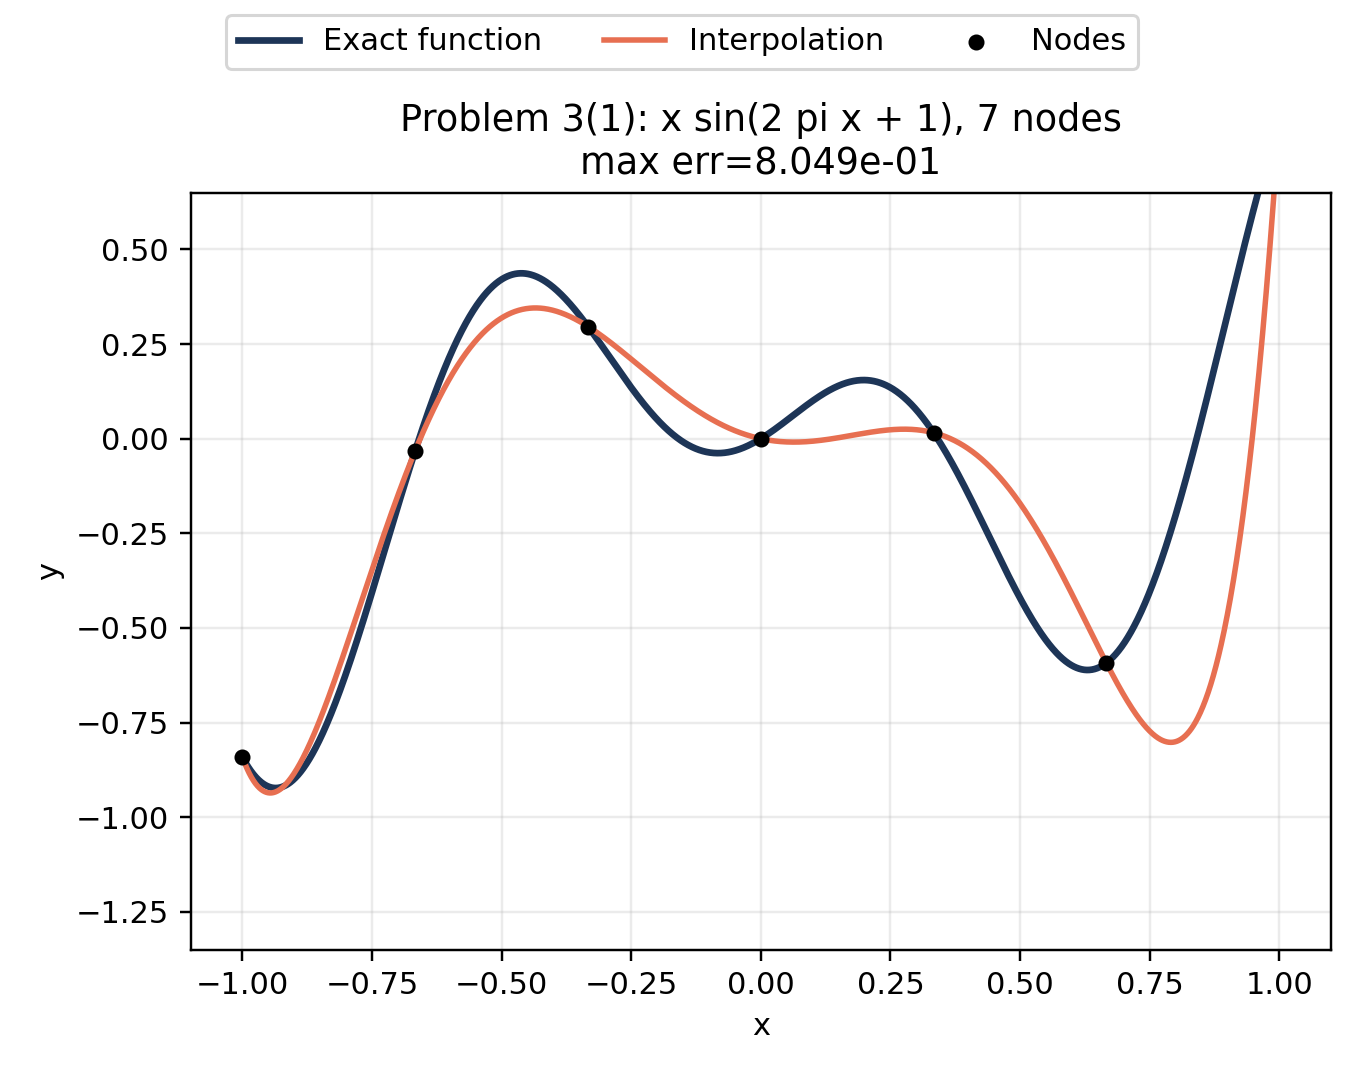
\includegraphics[width=0.94\linewidth]{problem3_sine_7_nodes.png}
  \caption{振荡函数 7 个等距节点插值结果。}
  \label{fig:p3_7}
\end{figure}

\begin{table}[H]
  \centering
  \caption{振荡函数 7 个节点插值误差。}
  \begin{tabular}{rrrr}
    \toprule
    节点数 & 插值次数 & 最大绝对误差 & RMSE \\
    \midrule
    7 & 6 & 8.048997e-01 & 2.465718e-01 \\
    \bottomrule
  \end{tabular}
\end{table}
从 \codeinline{7} 个节点的结果可以看出，初始插值已经能够大体跟随原函数，但边界附近仍存在较明显误差。该 6 次插值多项式的最大绝对误差为 \codeinline{8.048997e-01}，RMSE 为 \codeinline{2.465718e-01}；Neville 与重心 Lagrange 的最大逐点差异为 \codeinline{5.55e-16}，说明误差主要来自插值逼近本身。

\blocktitle{理解}
本小问作为基线实验，说明 \codeinline{7} 个等距节点下边界附近仍会出现可见偏差。它为下一小问观察误差随节点数 $b$ 增大而变化提供了基准。

\problem{Problem 3(2)：更多节点的重复实验}
\scriptlink{problem3.py}

\blocktitle{待求问题}
再对 \codeinline{9,17,19,21} 个节点重复，比较插值曲线与精确函数。

\blocktitle{解决方式}
本小问继续沿用 $m$ 个节点对应 $m-1$ 次插值的解释，并用 Neville 与重心 Lagrange 两种形式交叉核对。与 Runge 函数相比，本题目标函数在端点附近没有尖锐边界层，因此等距高阶插值的表现明显更好。这里的 $b$ 表示等距节点数。
提交包中，结果文件按题目和 Project 分组：Problem 1、Problem 2、Problem 3 分别归档到 \codeinline{results/problem1/}、\codeinline{results/problem2/}、\codeinline{results/problem3/}。Project 2 在 \codeinline{results/project2/} 内继续拆分为 \codeinline{output/}、\codeinline{manifest/}、\codeinline{benchmarks/} 与 \codeinline{references/ycruncher/}，避免大量 \codeinline{project2\_*} 文件堆在同一层。

\blocktitle{问题答案}
更多节点的插值结果见图~\ref{fig:p3_more}。其中 $b$ 表示等距节点数，最大误差与 RMSE 随 $b$ 增大的变化见图~\ref{fig:p3_error_b}。
\begin{figure}[H]
  \centering
  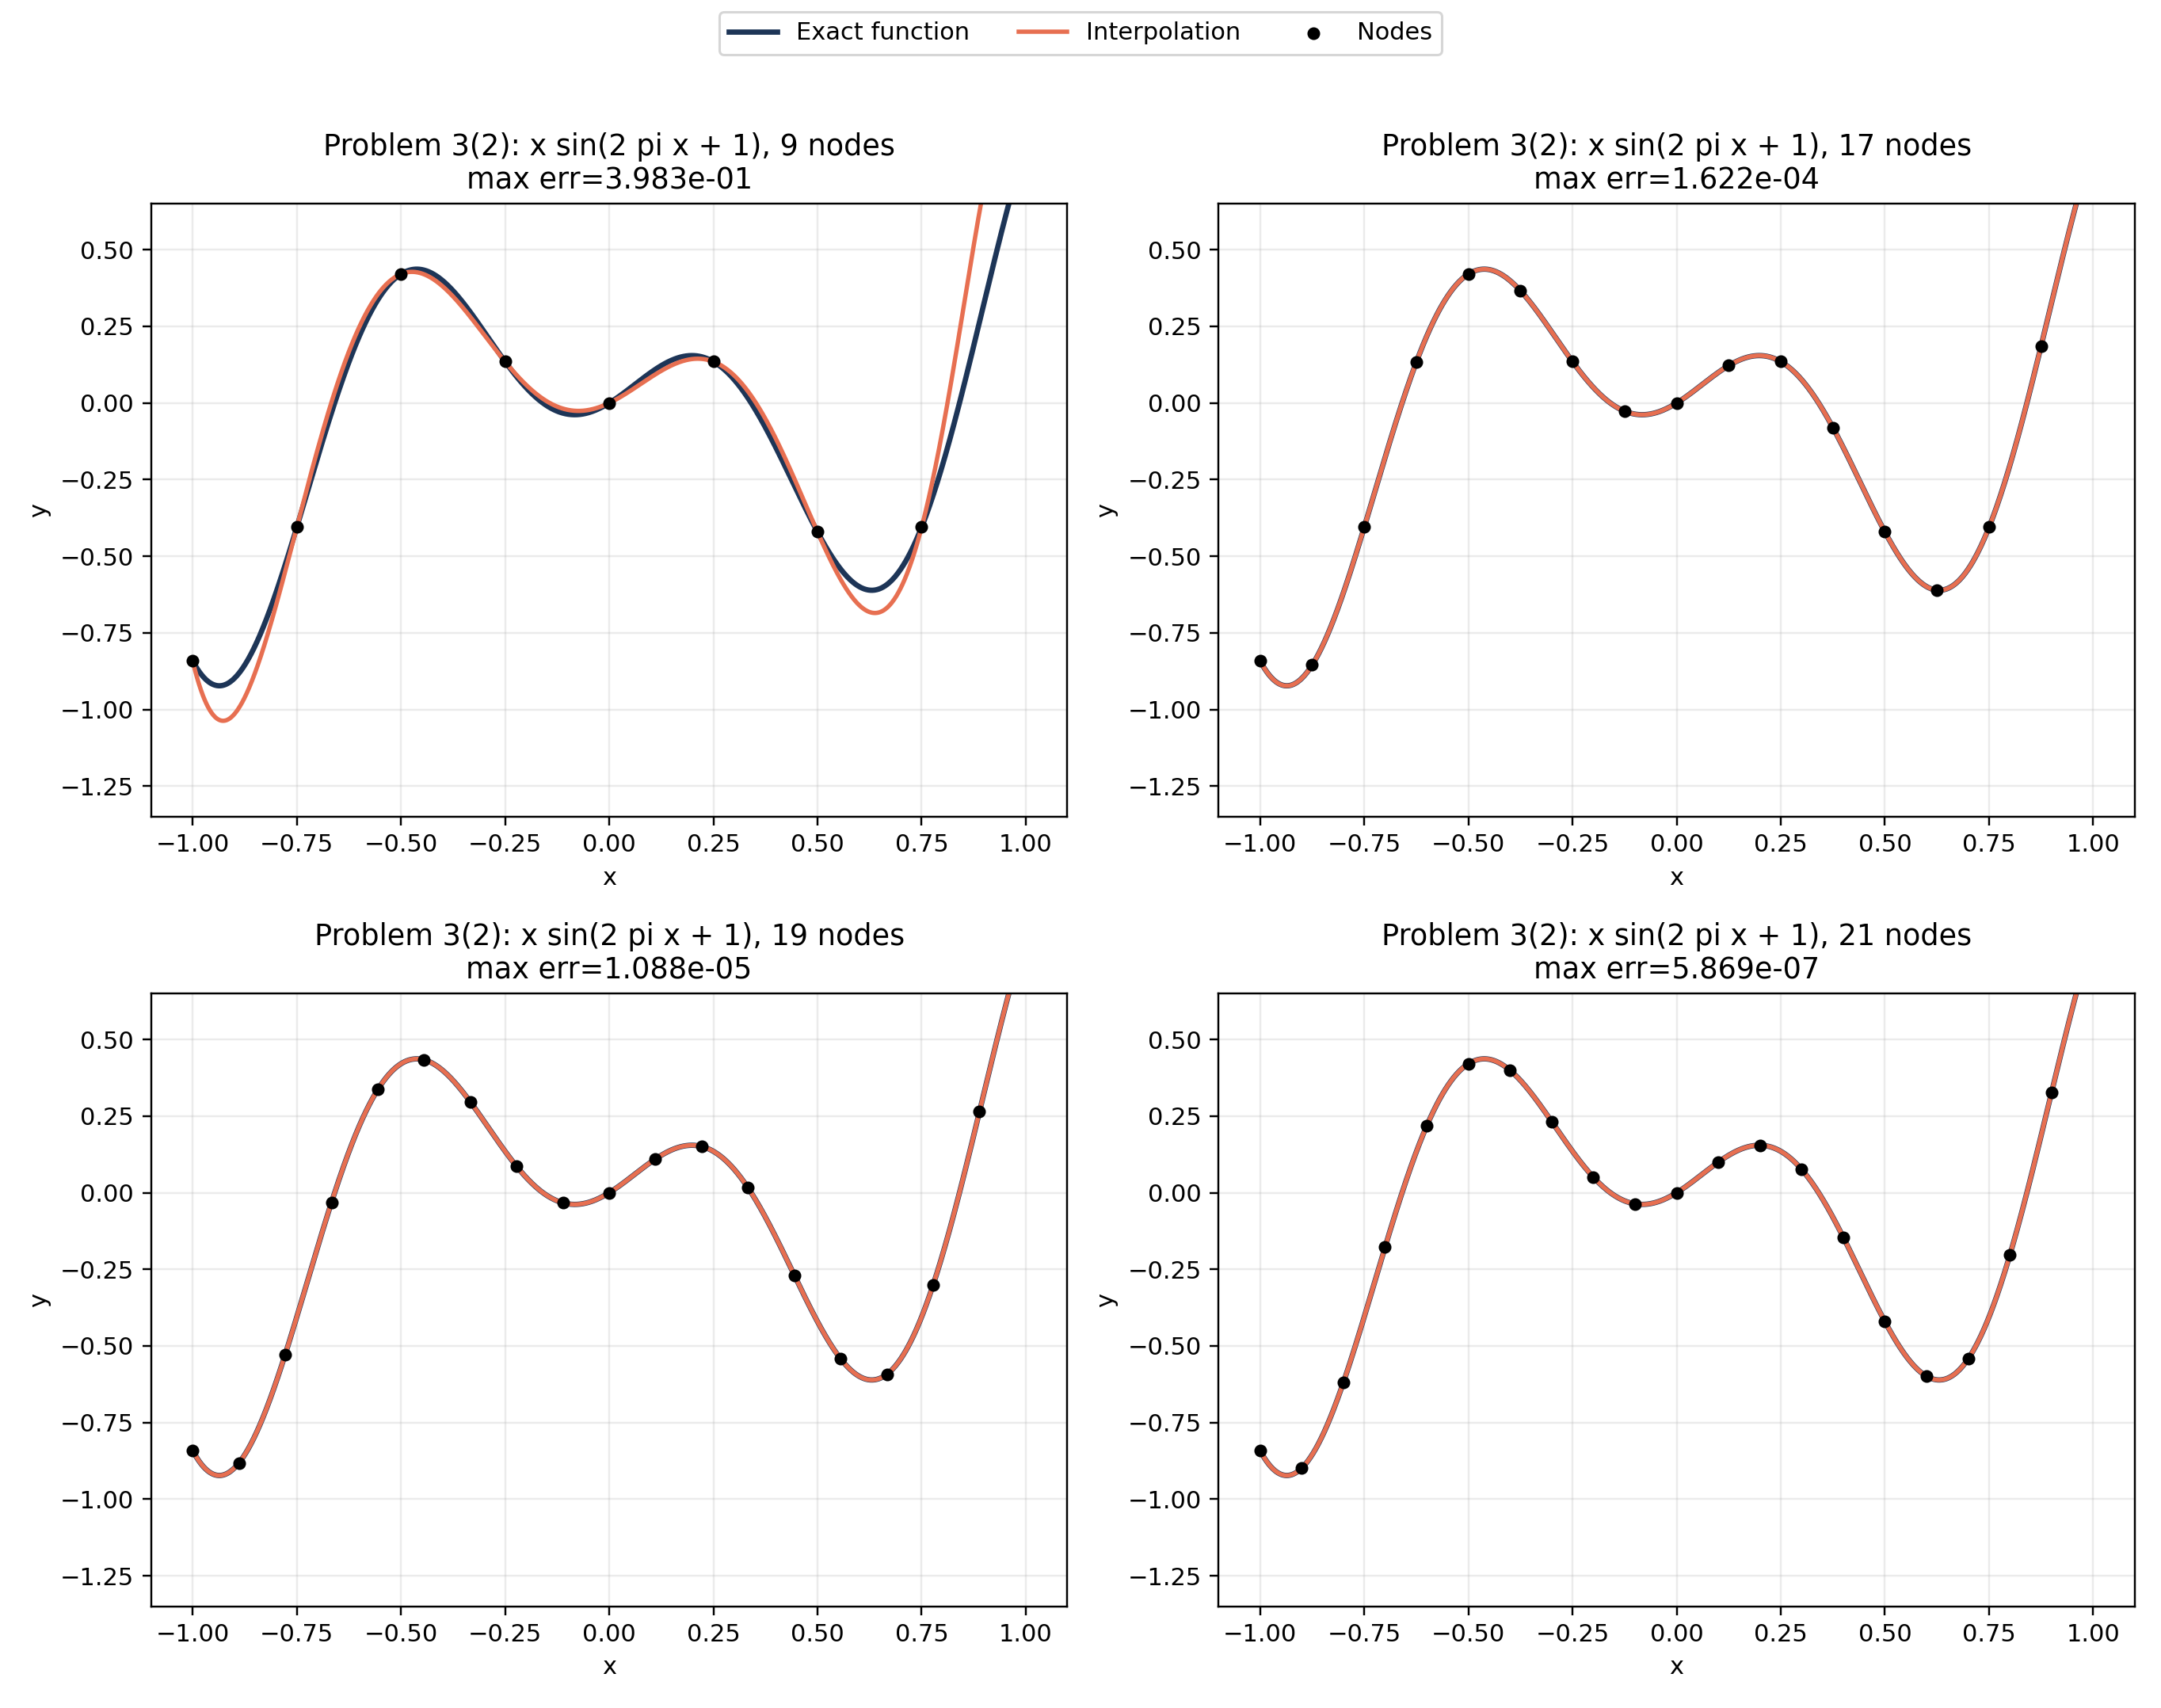
\includegraphics[width=0.99\linewidth]{problem3_sine_more_nodes.png}
  \caption{振荡函数更多等距节点插值结果。}
  \label{fig:p3_more}
\end{figure}

\begin{figure}[H]
  \centering
  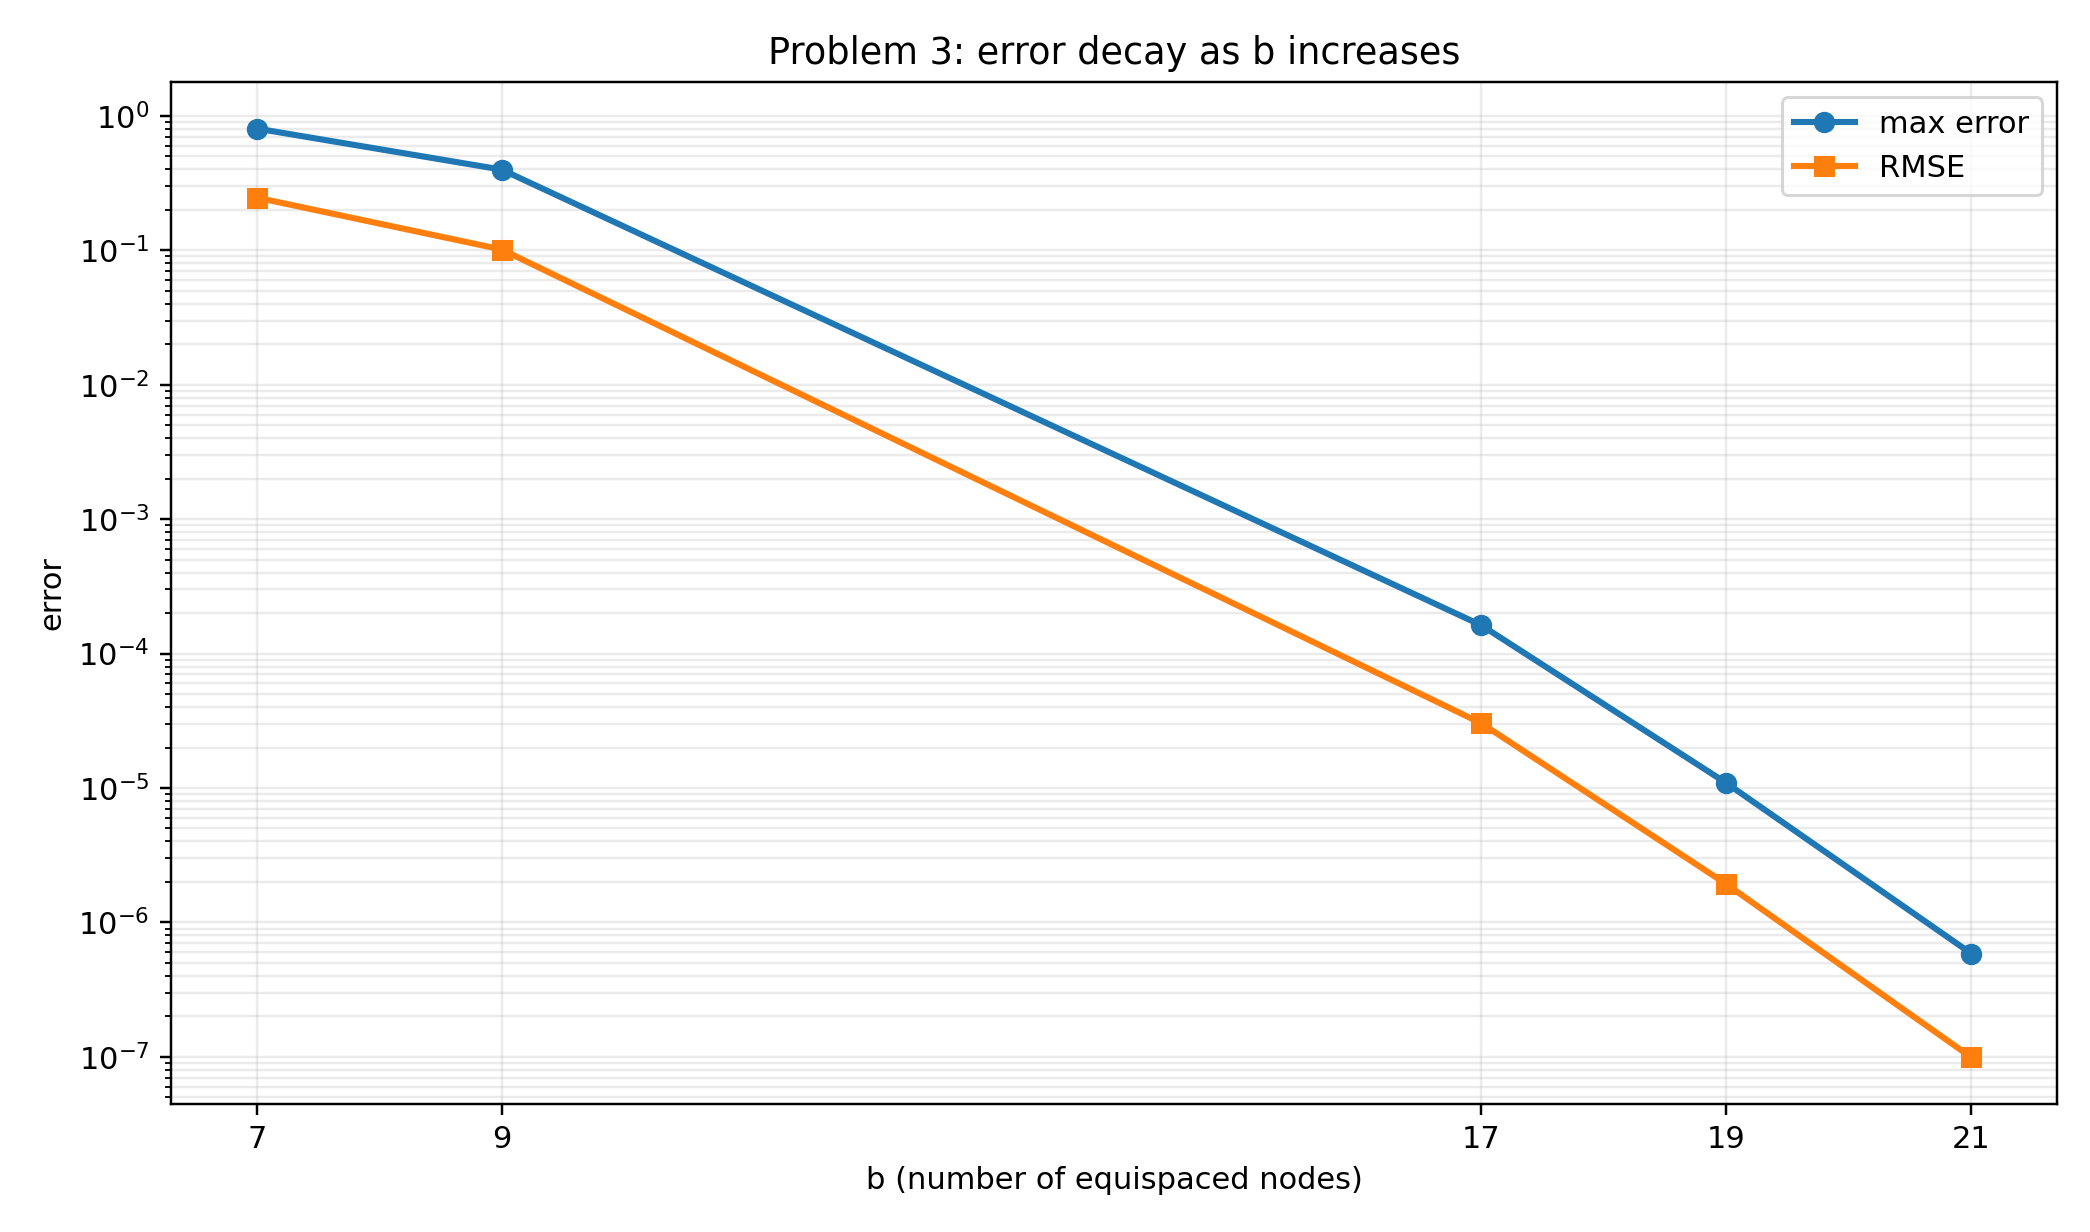
\includegraphics[width=0.90\linewidth]{problem3_sine_error_vs_b.png}
  \caption{振荡函数插值误差随节点数 $b$ 增大的变化。}
  \label{fig:p3_error_b}
\end{figure}

\begin{table}[H]
  \centering
  \caption{振荡函数更多节点插值误差。}
  \begin{tabular}{rrrr}
    \toprule
    节点数 & 插值次数 & 最大绝对误差 & RMSE \\
    \midrule
    9 & 8 & 3.983079e-01 & 1.014035e-01 \\
    17 & 16 & 1.621634e-04 & 3.026737e-05 \\
    19 & 18 & 1.088196e-05 & 1.927355e-06 \\
    21 & 20 & 5.868755e-07 & 9.914063e-08 \\
    \bottomrule
  \end{tabular}
\end{table}
继续增加节点数后，插值误差随次数提高而明显下降。\codeinline{21} 个节点时，最大绝对误差已降至 $5.87\times 10^{-7}$，相对于 \codeinline{7} 个节点约缩小 \codeinline{1.37e6} 倍；RMSE 从 \codeinline{2.465718e-01} 降至 \codeinline{9.914063e-08}，约缩小 \codeinline{2.49e6} 倍。图~\ref{fig:p3_error_b} 直接显示误差指标随 $b$ 增大而下降。

\blocktitle{理解}
这一结果与第二题形成鲜明对照。同样使用
\[
  f(x)-p_{b-1}(x)=\frac{f^{(b)}(\xi_x)}{b!}\omega_b(x)
\]
作为误差模型，差别主要来自目标函数。$x\sin(2\pi x+1)$ 是整函数，在复平面没有像 Runge 函数 $\pm i/4$ 那样贴近实轴的极点；它的高阶导数主要由三角函数频率 $2\pi$ 控制，并被插值误差公式中的 $b!$ 分母抵消。虽然等距节点仍然带来一定放大，但函数本身的可逼近性更强，误差衰减项压过了节点放大项。

对 \codeinline{b=7,9,17,19,21} 的误差作同样的半对数拟合得到
\[
  E_\infty(b)\approx 1.94\times10^{3}e^{-1.007b},\qquad
  E_2(b)\approx 7.52\times10^{2}e^{-1.048b},
\]
对应 $R^2$ 分别为 \codeinline{0.9864} 和 \codeinline{0.9888}。负指数系数给出了定量解释：每增加 1 个节点，最大误差平均约乘以 \codeinline{0.365}，RMSE 平均约乘以 \codeinline{0.351}。实际高阶段下降还更快，例如最大误差从 \codeinline{17} 到 \codeinline{19} 个节点约乘以 \codeinline{0.067}，从 \codeinline{19} 到 \codeinline{21} 个节点约乘以 \codeinline{0.054}。因此第三题不是“等距节点一定可靠”，而是该目标函数在本区间内足够平滑、没有近实轴奇点，使高阶多项式插值的逼近收益超过了等距节点的稳定性损失。

\reportgroup{IV. Project 2：高精度圆周率计算}

Project 2 要求在笔记本电脑上计算 $\pi$，精确到小数点后至少 \codeinline{10000} 位，并尽量兼顾两个目标：计算速度，以及可达到的位数规模。

\problem{Problem 4(1)：计算速度}
\scriptlink{problem4\_project2.py}

\blocktitle{待求问题}
尽量提高计算速度。

\blocktitle{解决方式}
主计算路线采用 Chudnovsky 公式与 binary splitting：
\begin{CodeBlock}
Input : target decimal digits d
Output: decimal expansion of pi and benchmark summary

N <- number of Chudnovsky terms required by d
(P, Q, T) <- binary_split(0, N)
s <- guard digits
X <- isqrt(10005 * 10^(2(d+s)))
pi_scaled <- floor(426880 * X * Q / T)
truncate guard digits and format decimal string

benchmark multiple backends:
    optimized CPU GMP route
    GPU hybrid route
    y-cruncher reference route
\end{CodeBlock}
速度比较分成两类：一类是自研路线在 \codeinline{10,000,000} 位上的同口径矩阵，另一类是 y-cruncher 在 \codeinline{100M/1B/2.5B} 位上的成熟工具链参考。二者目标位数不同，因此不把它们当作严格同规模对照；但它们共同回答“自研路线能达到什么速度”和“成熟工具链大约是什么量级”。

\blocktitle{问题答案}
若比较自研完整流水线，\codeinline{gpu\_hybrid\_merge\_fast\_auto} 在 \codeinline{10,000,000} 位上达到约 \codeinline{5.02e6 digits/s}，相对 \codeinline{cpp\_gmp\_openmp} 的 \codeinline{2.61e6 digits/s} 约快 \codeinline{1.92} 倍；作为成熟工具链参考，y-cruncher 在 \codeinline{100,000,000} 位上达到约 \codeinline{4.71e7 digits/s}。

\begin{table}[H]
  \centering
  \caption{Project 2 速度结果摘要。}
  \begin{tabular}{lrrr}
    \toprule
    路线 & 目标位数 & 用时 / s & 吞吐量 / digits/s \\
    \midrule
    Python+GMP & 10,000,000 & 4.754297 & 2.10e6 \\
    C++ GMP & 10,000,000 & 3.826070 & 2.61e6 \\
    C++ levelpool & 10,000,000 & 3.822220 & 2.62e6 \\
    GPU hybrid & 10,000,000 & 1.991292 & 5.02e6 \\
    y-cruncher & 100,000,000 & 2.124 & 4.71e7 \\
    y-cruncher & 1,000,000,000 & 26.042 & 3.84e7 \\
    y-cruncher & 2,500,000,000 & 73.693 & 3.39e7 \\
    \bottomrule
  \end{tabular}
\end{table}
表中自研路线均通过前缀核对；y-cruncher 三行分别有 \codeinline{Good through 100M}、\codeinline{Good through 1B} 与 \codeinline{Good through 2.5B} 的历史 validation 记录。

\blocktitle{理解}
Project 2 的速度问题不能只看 Chudnovsky 公式“每项约增加 14 位十进制有效数字”这一点。对 \(d\) 位计算，项数近似为 \(N\simeq d/14\)，例如 \codeinline{10,000,000} 位需要约 \codeinline{714,290} 项，\codeinline{100,000,000} 位需要约 \codeinline{7,142,861} 项。真正昂贵的部分不是逐项代入公式，而是随着位数增长而迅速变大的整数乘法、归并、平方根和最终除法。binary splitting 把级数写成三元组 $(P,Q,T)$ 的树形合并，避免在每一项上做高精度除法，并把大量工作转化为可并行的大整数乘法；因此它是本题能进入千万位乃至亿位规模的基础。

从 CPU 路线看，\codeinline{cpp\_gmp\_openmp} 与 \codeinline{cpp\_gmp\_levelpool} 在 \codeinline{10,000,000} 位上分别为 \codeinline{2.61e6} 与 \codeinline{2.62e6 digits/s}，两者几乎相同。这说明在当前规模下，单纯改变任务池组织方式已经不是主要矛盾；GMP 大整数乘法、树形归并和最终整除才是端到端时间的主体。Python+GMP 路线慢于 C++ 路线，也说明解释器调度和 Python 层对象组织会带来额外开销，但其数量级仍然由底层 GMP 支撑。

GPU hybrid 的意义在于把树形归并和最终大整数乘法中的一部分转到 GPU FFT 路线。表中 \codeinline{10,000,000} 位时它相对 C++ GMP 约快 \codeinline{1.92} 倍；在额外规模扫描中，\codeinline{20M/50M/100M} 位的 \codeinline{hybrid-fast-auto} 吞吐量约为 \codeinline{6.34e6/6.97e6/6.92e6 digits/s}，而对应 C++ CPU 路线约为 \codeinline{2.02e6/1.73e6/1.53e6 digits/s}，加速比随位数增大从约 \codeinline{3.15} 倍提高到约 \codeinline{4.52} 倍。这一趋势符合大整数乘法的特征：规模越大，FFT 类乘法和 GPU 并行吞吐越容易摊薄启动、传输和调度成本。

但是，GPU kernel 的峰值不能直接等同于圆周率端到端速度。单独的 GPU FFT 精确乘法在 \codeinline{100M} 量级可达到约 \codeinline{1.49e8 digits/s}，这是乘法内核吞吐信号；完整流水线还要做 chunk 生成、host-device 转换、树形归并、平方根、最终除法和十进制格式化。已有 profiling 中 \codeinline{100M} 运行的时间被分散到 partial generation、sqrt、merge tree、final division 等阶段，实际 GPU kernel 只占总流程的一部分。因此本题不能把“某个乘法 kernel 很快”写成“整个 $\pi$ 计算同样快”，而要以完整输出通过前缀或 manifest 校验的端到端时间为准。

y-cruncher 的结果则给出成熟工程实现的参考。它在 \codeinline{100M} 位上的 wall-time 吞吐约为 \codeinline{4.71e7 digits/s}，显著高于当前自研 hybrid 路线。这并不否定自研路线的有效性，而是说明 y-cruncher 在算法选择、汇编级乘法、内存调度、线程池和 NUMA/缓存利用上已经做了大量专门优化。自研路线的结论应表述为：已实现可复核的千万到亿位级计算，并在 GPU hybrid 下取得相对 CPU GMP 的明确加速；若以绝对最快为目标，成熟专用工具仍明显领先。

\problem{Problem 4(2)：已验证达到的位数规模}
\scriptlink{problem4\_project2.py}

\blocktitle{待求问题}
尽量提高可达到的位数规模，且至少达到小数点后 \codeinline{10000} 位。本文只报告已经生成并验证的自研输出规模，不声称完成了位数极限测试。

\blocktitle{解决方式}
位数规模的验证不再强调各后端速度，也不把历史大位数记录解释为当前自研代码的极限；本小问只确认提交包中已有输出是否确实超过题目要求。主计算路线仍采用 Chudnovsky 公式与 binary splitting：
\begin{CodeBlock}
Input : target decimal digits d
Output: decimal expansion of pi and benchmark summary

N <- number of Chudnovsky terms required by d
(P, Q, T) <- binary_split(0, N)
s <- guard digits
X <- isqrt(10005 * 10^(2(d+s)))
pi_scaled <- floor(426880 * X * Q / T)
truncate guard digits and format decimal string

validate output:
    write 100,000,000 decimal digits
    compute byte size and file fingerprint
    record first, last, fixed-offset and deterministic sample windows
    compare historical y-cruncher validation logs
\end{CodeBlock}
完整高精度结果以 \codeinline{100M} 位十进制文本保存，提交包中放在 Project 2 的 \codeinline{output/} 子目录；复核入口 \codeinline{make project2\_manifest} 只读取已有文件，并把 sidecar 写入 \codeinline{manifest/}。该入口不触发重算；历史 y-cruncher benchmark、日志与 validation 文件放在 \codeinline{references/ycruncher/} 下，只作为外部工具参考，不作为自研代码可达极限的证据。

\blocktitle{问题答案}
精度方面，题目所要求的 \codeinline{10000} 位已经被大幅超越，本次报告已经验证到 \codeinline{100000000} 位完整十进制输出，是题目最低要求的 \codeinline{10000} 倍。这个数值是本次自研结果的已验证达到规模，也是当前报告能够给出的保守下界；它不是位数极限。

\blocktitle{理解}
这一小问的核心不是“程序能打印很多字符”，而是这些字符是否能证明为同一次高精度计算的有效输出。题目最低要求是小数点后 \codeinline{10000} 位，当前提交的自研输出为小数点后 \codeinline{100000000} 位，规模上超过最低要求 \codeinline{10000} 倍。文件大小 \codeinline{100000003 bytes} 与格式也相互一致：\codeinline{3.} 占 2 字节，后面有 \codeinline{100000000} 个小数位，最后换行占 1 字节。这个简单的大小关系可以排除明显截断或多余内容，但还不足以证明内容正确。

因此报告使用 manifest 作为结果可信性的主证据。manifest 中的文件哈希是机器校验用的文件指纹，不是人工阅读的数值结论；它用于固定完整文件的逐字节内容，便于之后确认提交包里的大文件没有被替换或截断。首段、末段、25M、50M、75M 等固定偏移窗口说明文件不是只在开头正确；确定性抽样窗口进一步降低了“中间大段被替换但未被发现”的风险。前 \codeinline{69} 位匹配圆周率已知前缀只是轻量 sanity check，不能单独证明 \codeinline{100M} 位全正确；它必须和文件指纹、窗口抽样以及外部 validation 记录结合使用。

因此，本小问的结论应是“已验证自研输出达到 \codeinline{100M} 位”，而不是“已经测得本机或本程序的位数极限”。真正的极限规模需要专门设计递增位数实验，记录每个目标位数的成功、失败、内存峰值、运行时间和失败原因；当前报告没有做这样的极限搜索。Chudnovsky 公式的收敛速度本身并不是主要限制，实际限制来自大整数乘法、binary splitting 树中最大操作数、内存峰值、I/O 和验证成本。由于缺少完整的递增位数失败边界，\codeinline{100M} 只能作为当前自研结果的保守可达下界。

y-cruncher 的 \codeinline{1B} 与 \codeinline{2.5B} validation 记录只能说明成熟工具链在本机环境中有过更大规模参考结果，不能替代自研代码的位数测试。报告中把二者分开，是为了避免把外部工具记录混入自研结果的证据链。默认 manifest 目标只读取既有输出并生成哈希和抽样证据，不触发大位数重算，这样既保留了可复核性，也避免把高成本实验隐藏在普通构建流程中。

\end{document}
